\subsection{Results and discussion}


The combination procedure is performed for each of the two PDF sets
taken into consideration at NNLO and at NNLO+NNLL separately. The
combination results and their unweighted average are displayed
numerically in Table~\ref{tab:combinationresults}, and graphically in
Fig.~\ref{fig:unweightedaverage}.

There is no unique way to quote a final best estimate of $\as$ based
on the results obtained from the different PDF sets and QCD
calculation choices (NNLO v.\ NNLO+NNLL).
%
An unbiased approach for combining results from different PDFs, in
line with the PDF4LHC recommendations~\cite{Butterworth:2015oua}, is to average
without applying any further weighting.
%
In accordance with that approach we take the straight average of the mean
values and the uncertainties of the individual combinations.
%
This coincides with the procedure for combining $\as$ results from a
single class of observables in Ref.~\cite{pdg}.
%
The final result is
\begin{equation}
\asmz =
    \alphasResultCenter
    \; {}^{\highersub{$+\alphasResultRightError${}}}_{\lowersub{$-\alphasResultLeftError${} }}
\end{equation}
%
which can be compared to the result of Ref.~\cite{Chatrchyan:2013haa},
$\as(m_Z) = 0.1151^{+0.0028}_{-0.0027}$.
%
Our central value is larger mainly because recent measurements of the
cross sections are higher than that used in
Ref.~\cite{Chatrchyan:2013haa}, but also in part because of our choice
to take the average of results from NNLO and NNLO+NNLL cross sections
(a $0.6\%$ increase relative to just NNLO+NNLL).
%
Our symmetrised uncertainty of $\alphasResultSymmPercentage\%$ is
somewhat increased with respect to that of
Ref.~\cite{Chatrchyan:2013haa}, $2.4\%$ (symmetrised).
%
The difference in uncertainty is due to several choices.
%
On one hand we have taken a smaller uncertainty on the top-quark mass,
in line with the PDG determination.
%
One the other hand, we have been somewhat more conservative in our
treatment of theoretical and PDF uncertainties.
%
Firstly, the choice of treating the scale uncertainties on $\stt$ as a
$68\%$ confidence interval instead of a (flat) $100\%$ confidence
interval increases the scale uncertainty component by roughly a factor
of $\sqrt{3}$.
%
Secondly, we have used an average of the uncertainties from NNLO and
NNLO+NNLL cross section determinations, which also yields a larger
uncertainty than using NNLO+NNLL cross section determinations only.
%
Finally, the PDF sets used for the determination were chosen with
minimization of potential biases in mind, rather than the ones with
smallest uncertainty.
%


\begin{table*}[ht] 
{\scriptsize  
\renewcommand{\arraystretch}{1.4}
\renewcommand{\ErrTableWidth}{0.6cm}
\begin{center} 
\hspace*{-0.75cm}\begin{tabular}{l c c c c c c c c c }
\toprule
& 
\cell{\ErrTableWidth}{Center} & 
\cell{\ErrTableWidth}{Stat.} & 
\cell{\ErrTableWidth}{Syst.} & 
\cell{\ErrTableWidth}{$E_{\text{beam}}$} & 
\cell{\ErrTableWidth}{Lumi.} & 
\cell{\ErrTableWidth}{$\mt$} & 
\cell{\ErrTableWidth}{PDF} & 
\cell{\ErrTableWidth}{Scale} & 
\cell{\ErrTableWidth}{Total} \\ 
\midrule
CT14 {\tiny (NNLO)}            & $0.1184$ & ${}_{-0.0003}^{+0.0003}$ & ${}_{-0.0007}^{+0.0006}$ & ${}_{-0.0001}^{+0.0001}$ & ${}_{-0.0006}^{+0.0006}$ & ${}_{-0.0014}^{+0.0010}$ & ${}_{-0.0023}^{+0.0016}$ & ${}_{-0.0025}^{+0.0025}$ & ${}_{-0.0038}^{+0.0033}$ \\
NNPDF30\_nolhc {\tiny (NNLO)}  & $0.1182$ & ${}_{-0.0003}^{+0.0003}$ & ${}_{-0.0007}^{+0.0007}$ & ${}_{-0.0000}^{+0.0000}$ & ${}_{-0.0007}^{+0.0007}$ & ${}_{-0.0013}^{+0.0012}$ & ${}_{-0.0025}^{+0.0023}$ & ${}_{-0.0026}^{+0.0031}$ & ${}_{-0.0040}^{+0.0042}$ \\
CT14 {\tiny (NNLO+NNLL)}       & $0.1172$ & ${}_{-0.0003}^{+0.0003}$ & ${}_{-0.0007}^{+0.0007}$ & ${}_{-0.0001}^{+0.0001}$ & ${}_{-0.0007}^{+0.0006}$ & ${}_{-0.0014}^{+0.0011}$ & ${}_{-0.0023}^{+0.0017}$ & ${}_{-0.0017}^{+0.0015}$ & ${}_{-0.0033}^{+0.0027}$ \\
NNPDF30\_nolhc {\tiny (NNLO+NNLL)} & $0.1168$ & ${}_{-0.0003}^{+0.0003}$ & ${}_{-0.0007}^{+0.0006}$ & ${}_{-0.0001}^{+0.0001}$ & ${}_{-0.0007}^{+0.0007}$ & ${}_{-0.0013}^{+0.0012}$ & ${}_{-0.0024}^{+0.0023}$ & ${}_{-0.0017}^{+0.0018}$ & ${}_{-0.0034}^{+0.0033}$ \\
\midrule
Average                        & $0.1177$ & ${}_{+0.0003}^{+0.0003}$ & ${}_{+0.0007}^{+0.0007}$ & ${}_{+0.0001}^{+0.0001}$ & ${}_{+0.0007}^{+0.0006}$ & ${}_{+0.0013}^{+0.0012}$ & ${}_{+0.0024}^{+0.0020}$ & ${}_{+0.0021}^{+0.0022}$ & ${}_{-0.0036}^{+0.0034}$ \\
\bottomrule
\end{tabular} 
\end{center} 
\caption{\small Combination results for all PDF sets taken into consideration, at NNLO and NNLO+NNLL.}
\label{tab:combinationresults}
} 
\end{table*} 


\newcommand{\ScanFigureWidth}{0.47}  
\begin{figure}[htb]
\centering
\begin{tabular}{ccc}
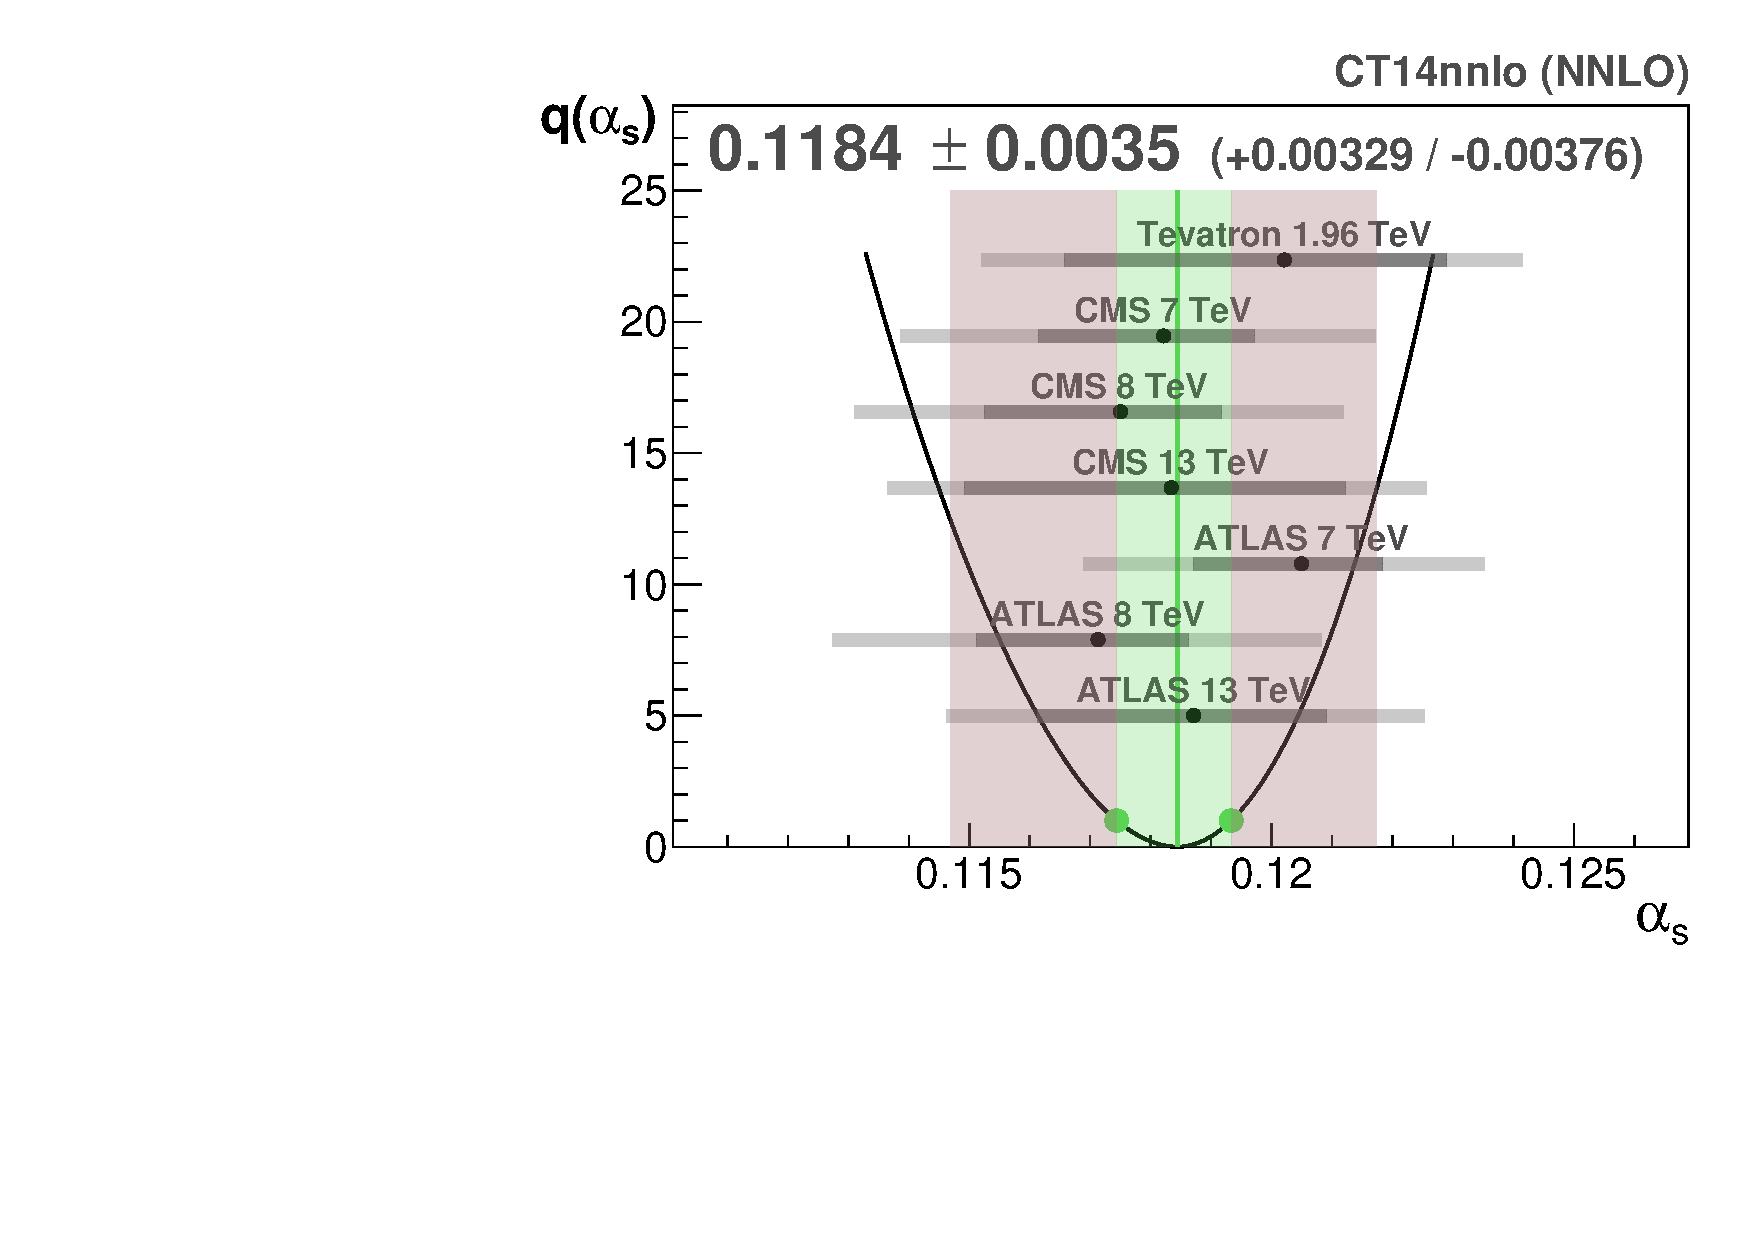
\includegraphics[width=\ScanFigureWidth\linewidth]{%
    img/alphas/ScanResult_likelihood_asym_2step_NNLO-CT14nnlo.pdf%
    }
&
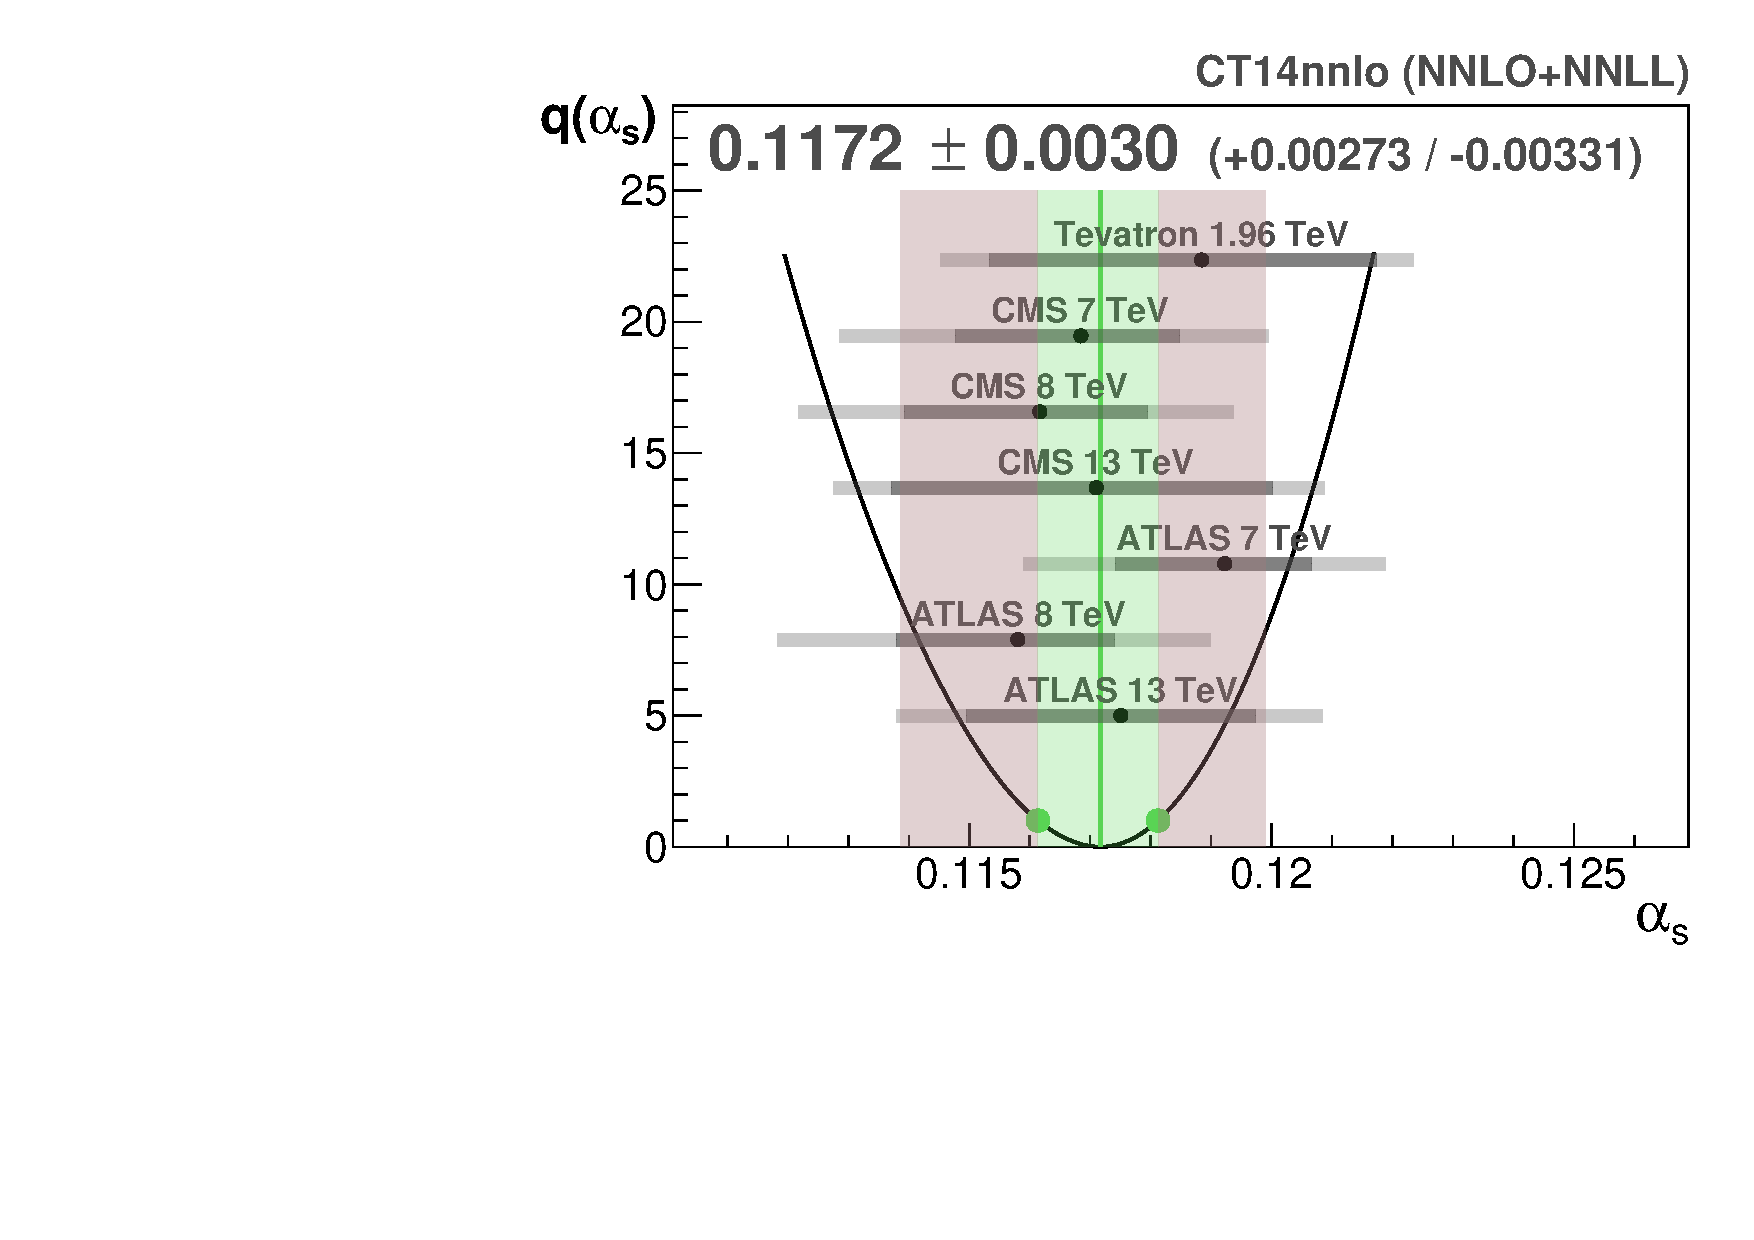
\includegraphics[width=\ScanFigureWidth\linewidth]{%
    img/alphas/ScanResult_likelihood_asym_2step_NNLO-NNLL-CT14nnlo.pdf%
    }
\\[-6pt]
(a) & (b) \\[8pt]
%
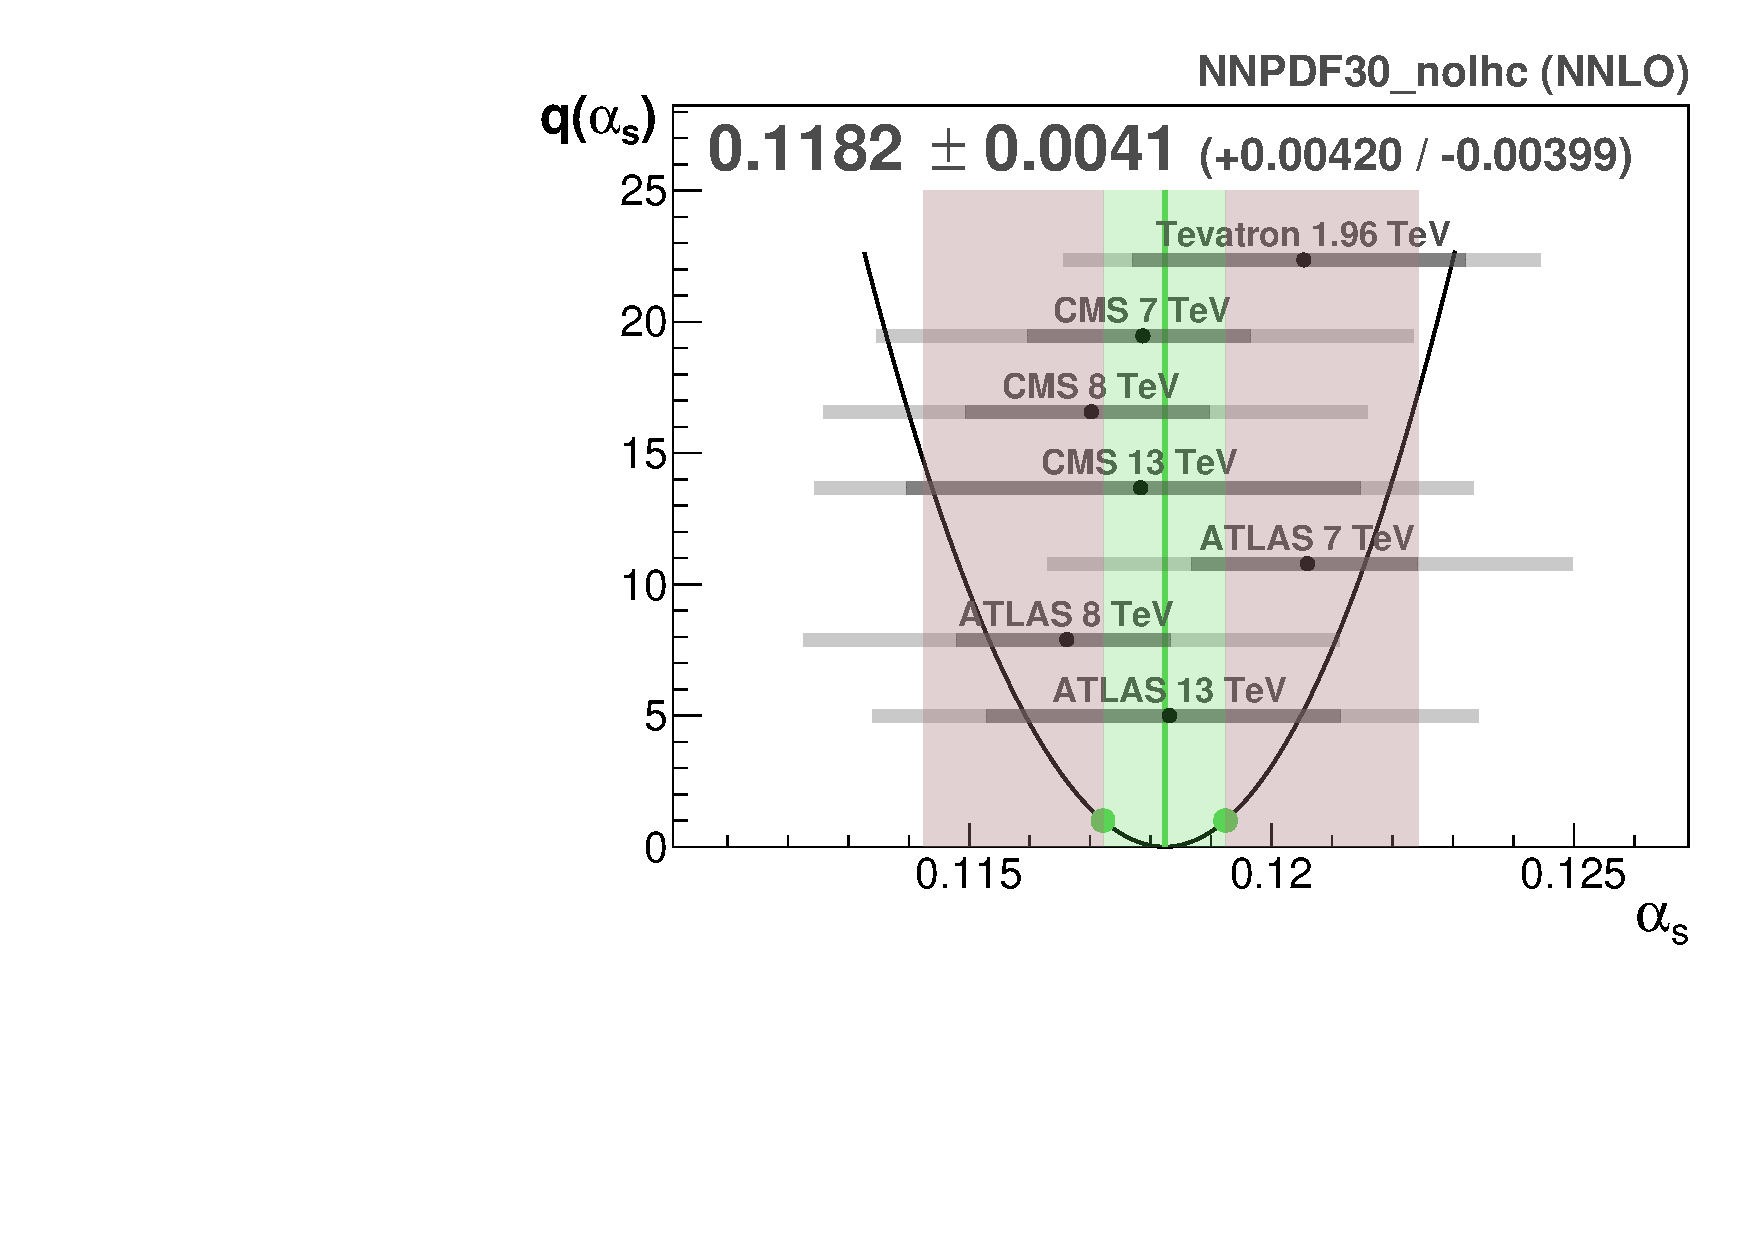
\includegraphics[width=\ScanFigureWidth\linewidth]{%
    img/alphas/ScanResult_likelihood_asym_2step_NNLO-NNPDF30-nolhc-nnlo.pdf%
    }
&
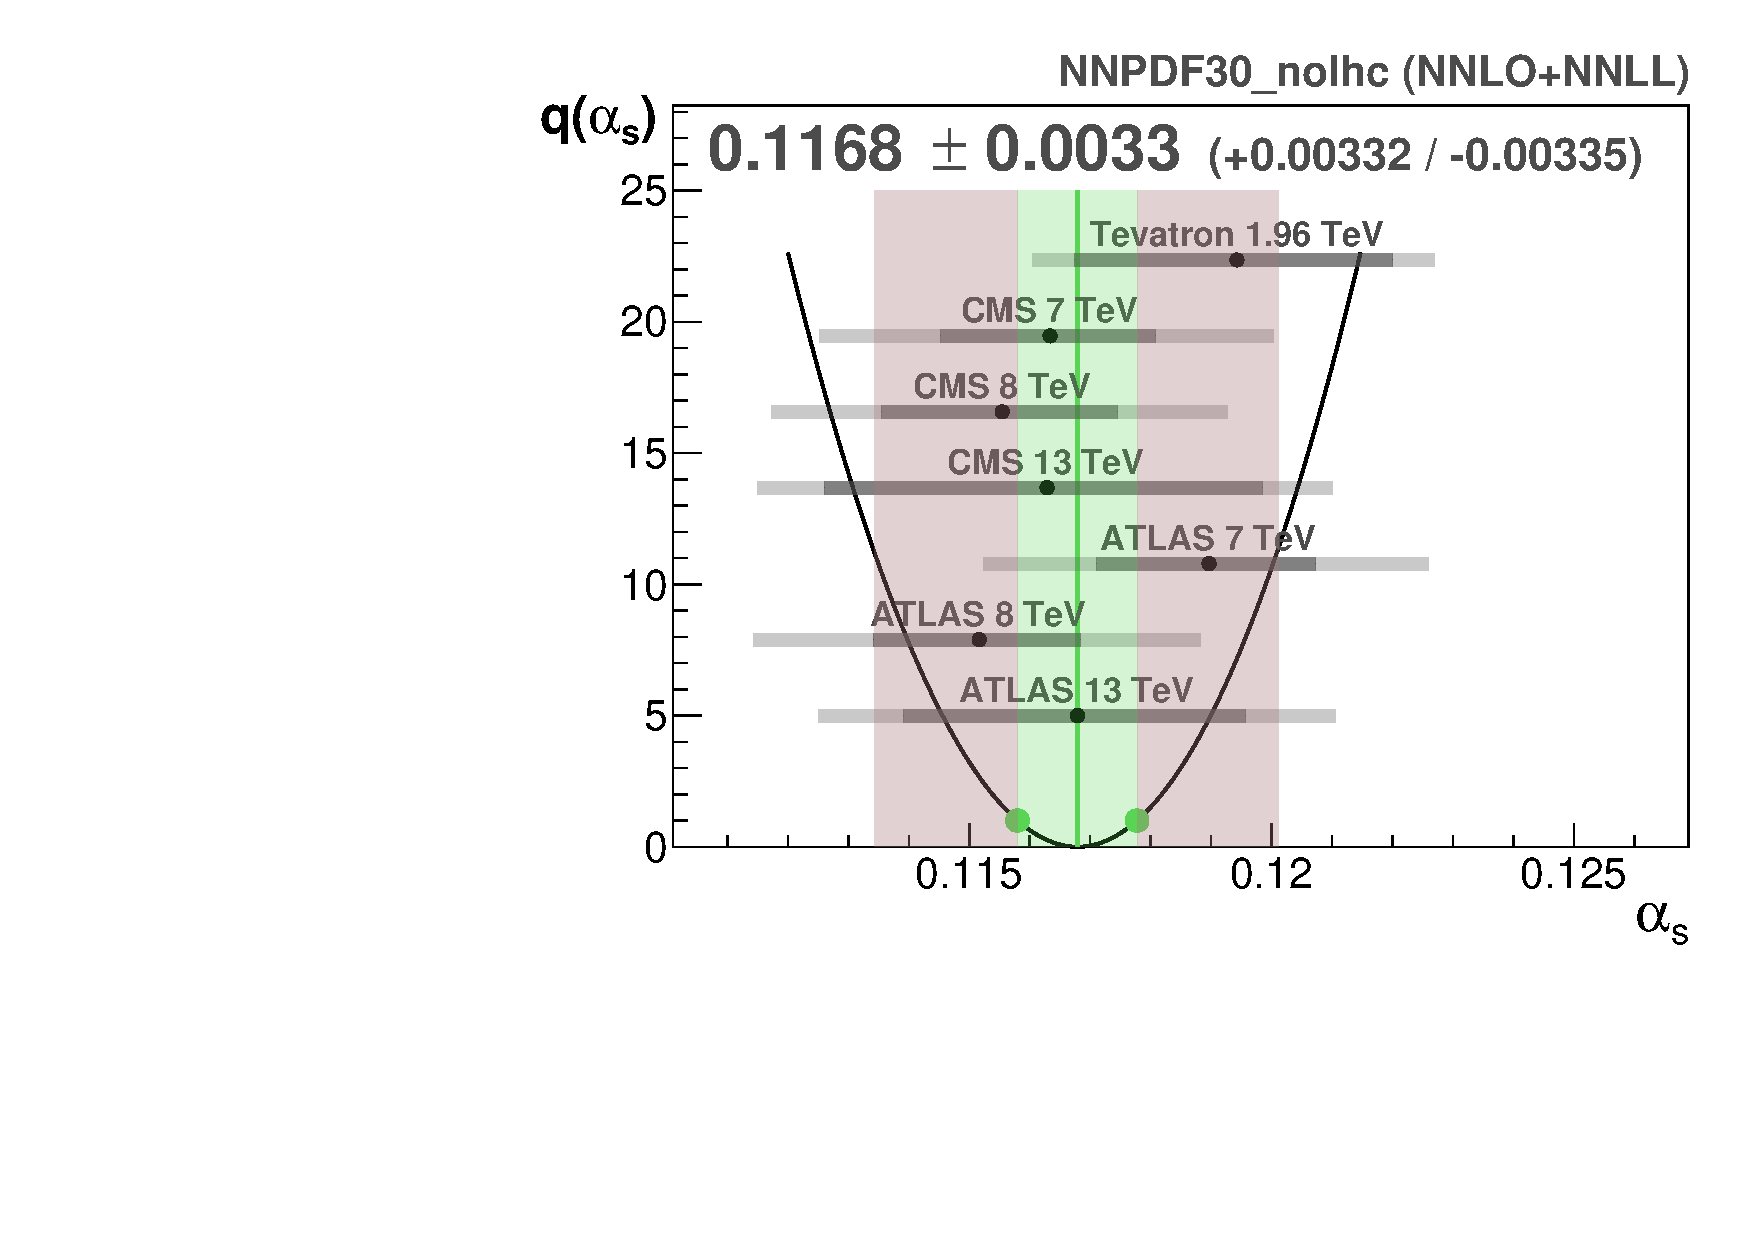
\includegraphics[width=\ScanFigureWidth\linewidth]{%
    img/alphas/ScanResult_likelihood_asym_2step_NNLO-NNLL-NNPDF30-nolhc-nnlo.pdf%
    }
\\[-6pt]
(c) & (d) \\[6pt]
\end{tabular}
\vspace{-0.3cm}
\caption{
Combination results using the CT14 PDF set (NNLO in (a) and NNLO+NNLL in (b)) and the NNPDF3.0 noLHC PDF set (NNLO in (c) and NNLO+NNLL in (d)).
%
The individual determinations and their uncertainties are shown in grey, where the darker shade represents the experimental uncertainties which enter into the combination.
The test statistic $q$ as a function of $\as$ is plotted as a black line.
The green line and band represent the central value of the combination and the $1\sigma$ confidence interval respectively. 
The red band depicts the total combination uncertainty with scale, PDF
and top-mass uncertainties included.
}
\label{fig:ScanResults}
\end{figure}
% 
%
\begin{figure}[htb]
\centering
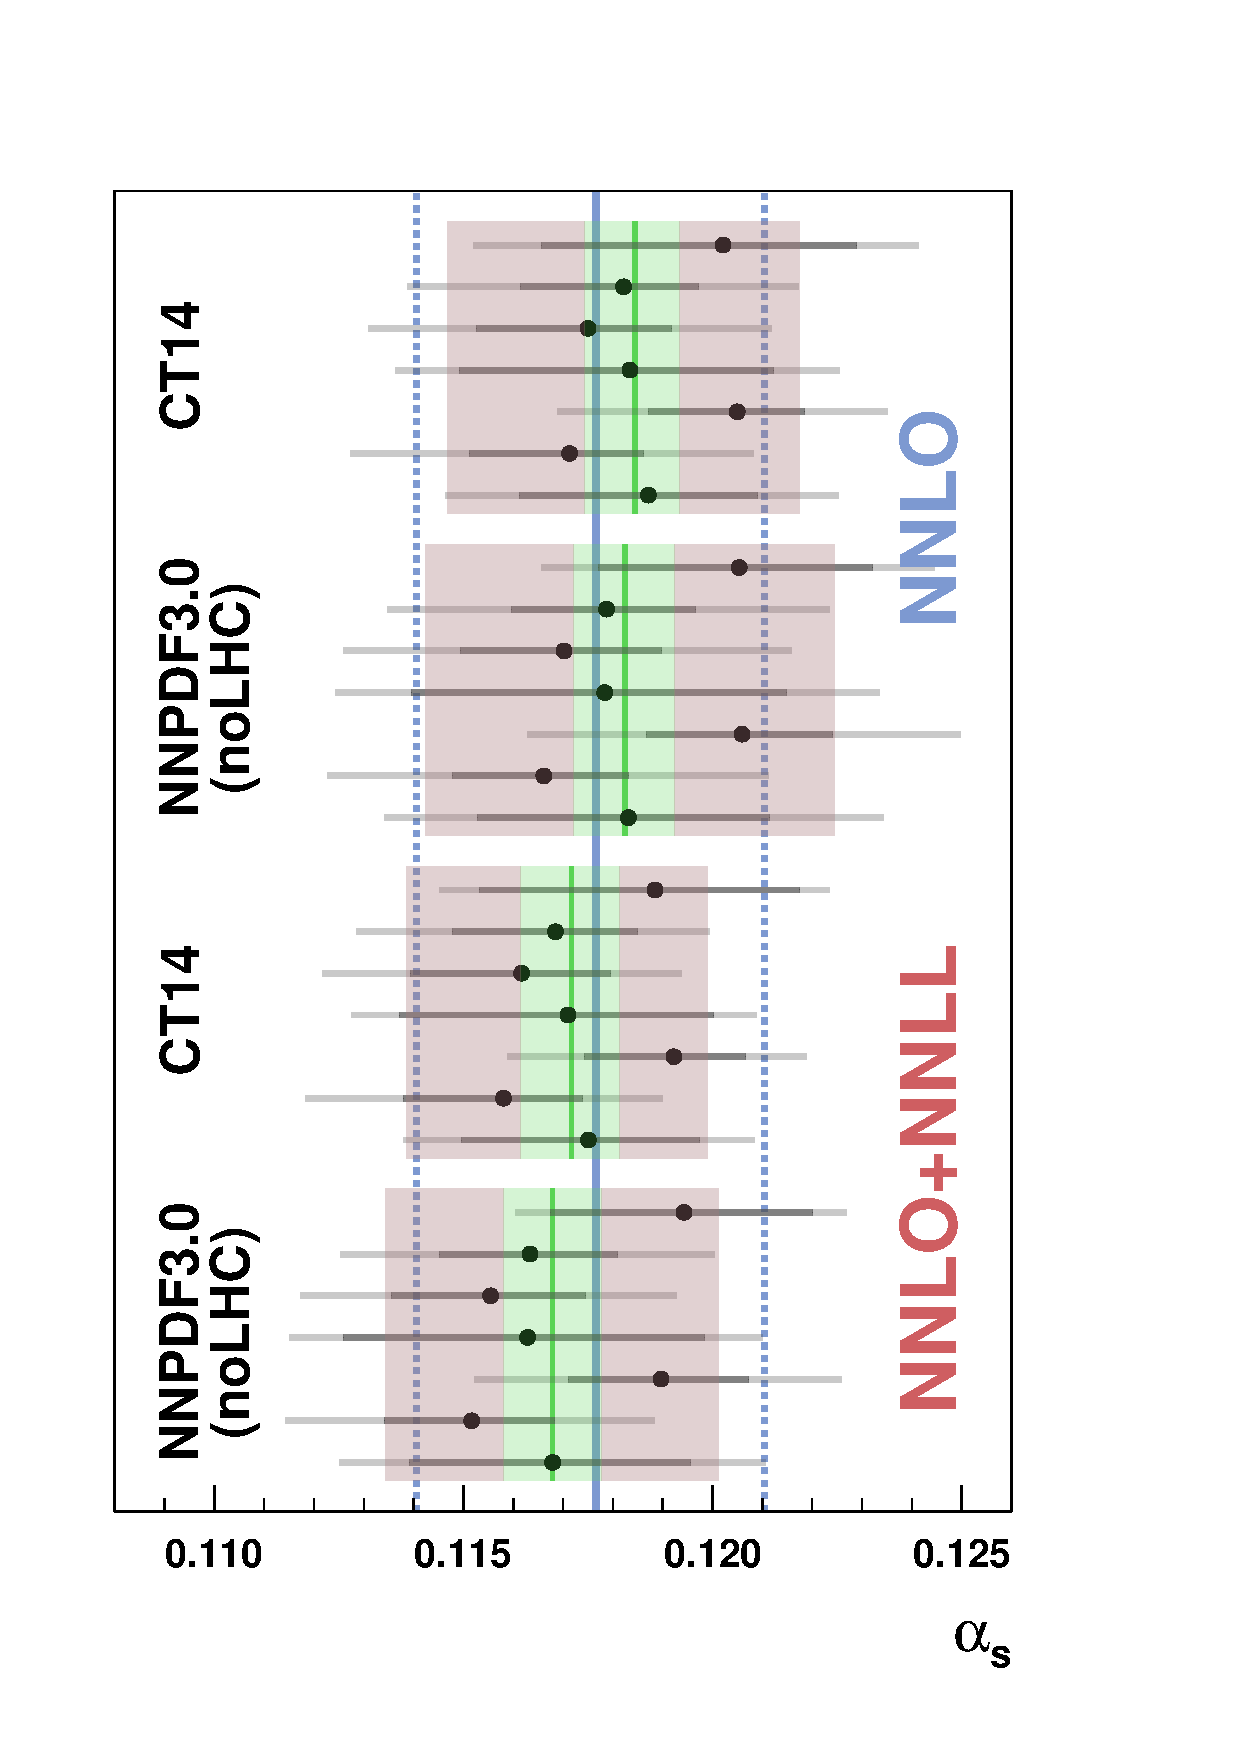
\includegraphics[width=0.6\linewidth]{img/alphas/summaryPlot_Collection_bfins_Jul05.pdf}
\vspace{-0.3cm}
\caption{
Combination results for all PDF sets taken into consideration, at NNLO
and NNLO+NNLL. The solid blue line is the unweighted average of the
individual combination results, and the dashed blue lines represent
the 68\% confidence interval.
%
The red and green bands are as in Fig.~\ref{fig:ScanResults}.
%
}
\label{fig:unweightedaverage}
\end{figure}

